\chapter{Разработка  Прототипа атомно-зондового томографа с лазерным испарением}\label{ch:ch2}

Разработки атомно-зондовой томографии в ИТЭФ (Россия) получили развитие в связи с модернизацией Центра атомно-масштабных и ядерно-физических микроскопических исследований конденсированных сред для получения разносторонней информации о наномасштабном состоянии различных материалов КАМИКС, включенного в перечень уникальных установок уникальных ядерно-физических установок, необходимых для осуществления национальным исследовательским центром «Курчатовский институт» своей деятельности (Распоряжение от 30 декабря 2009 г. №2125-р). Для расширения спектра исследований, проводящихся в ИТЭФ, в 2011 г. было принято решение о начале разработки стенда атомно-зондовой томографии нового поколения. В 2015 г. в ИТЭФ был запущен томографический атомный зонд с лазерным испарением и прямопролетной \cite{scbibAPPLE}. Установка получила сокращенное название ПАЗЛ-3D – Прототип Атомного Зонда с Лазерным испарением. 

\section{Общая схема установки}\label{sec:ch2/sec1}

Как уже было сказано в первой главе наиболее значимым различием между конфигурациями установок АЗТ является выбранный тип испарения. Если используется сугубо полевой тип испарения, то появляется необходимость использовать различного рода системы компенсации энергий ионов. Это значительно усложняет разработку установки, а также требует наличия дополнительного узла и сложный расчет взаиморасположения образца, испаряющего контр-электрода, системы компенсации энергий ионов и детектирующей системы. Для разработки ПАЗЛ-3D было выбрано испарение с помощью лазерной системы, для которого достаточно прямо-пролетной геометрии. Также прямо-пролетная геометрия обеспечивает в общем случае больший угол сбора данных, чем системы с рефлектроном (за исключением систем типа "сферическое зеркало"). Надо отметить, что выбор испарения с помощью лазера накладывает дополнительные требования по вводу лазерного излучения внутрь анализационного объема и взаиморасположения окна для лазера и образца, так как необходимо прямое попадание лазерного излучения на кончик образца.
Выбранная прямо-пролетная геометрия позволяет довольно легко оценить порядок разрешения по массе при разработке. Для разрабатываемой системы разрешение оп массе можно оценить используя формулу \cref{eq:equation8}. Ниже в Таблице \cref{tab:calcFWHM} приведены значения разрешения по массе для иона массой 30 а.е.м., с разбросом измерения времени пролета в 0,5 нс и в 1 нс. Выбранные наименьший и наибольший разбросы измерения времени пролета ионов для оценки верхней и нижней границ разрешения по массе для разрабатываемого прибора. С учетом выбора стандартных комплектующих вакуумной системы установки, расстояние между кончиком образца и детектором в ПАЗЛ-3D составляет 183 мм.

\begin{table} [htbp]
	\centering
	\caption{Сравнение разрешения по массе для иона при различных ускоряющих напряжения на образце}
	\label{tab:calcFWHM}
	\begin{SingleSpace}
		\begin{tabular} {| c | c | c | c |}
			\hline
			Длина пролета, мм & \thead{Разброс времени\\ пролета, нс} & Напряжение, кВ & \thead{Разрешение \\по массе, отн. ед.}  \\ \hline
			183 & 1 & 1  &  570               \\ \hline
			183 & 1 & 3  &  329               \\ \hline
			183 & 1 & 5  &  255               \\ \hline
			183 & 1 & 10 &  180               \\ \hline
			183 & 0,5 & 1  &  1140               \\ \hline
			183 & 0,5 & 3  &  658               \\ \hline
			183 & 0,5 & 5  &  510               \\ \hline
			183 & 0,5 & 10 &  360               \\ \hline
		\end{tabular}
	\end{SingleSpace}
\end{table}

Как видно из Таблицы \cref{tab:calcFWHM} установка АЗТ ПАЗЛ-3D в идеальных условия будет способна различать пики на масс-спектре отстоящие друг от друга на расстоянии от 0,01 а.е.м до 0,08 а.е.м. Такое качество масс-спектра более чем достаточно для распознания практически любых элементов и их изотопов. Полученное разрешение по массе соответствует разрешению по массе зарубежных установок аналогичной конфигурации.
На Рисунке \cref{fig:main_scheme} представлена общая схема расположения образца, детектирующей системы, криогенной системы и лазерной системы в ПАЗЛ-3D.
\begin{figure}[htb]
	\centerfloat{
		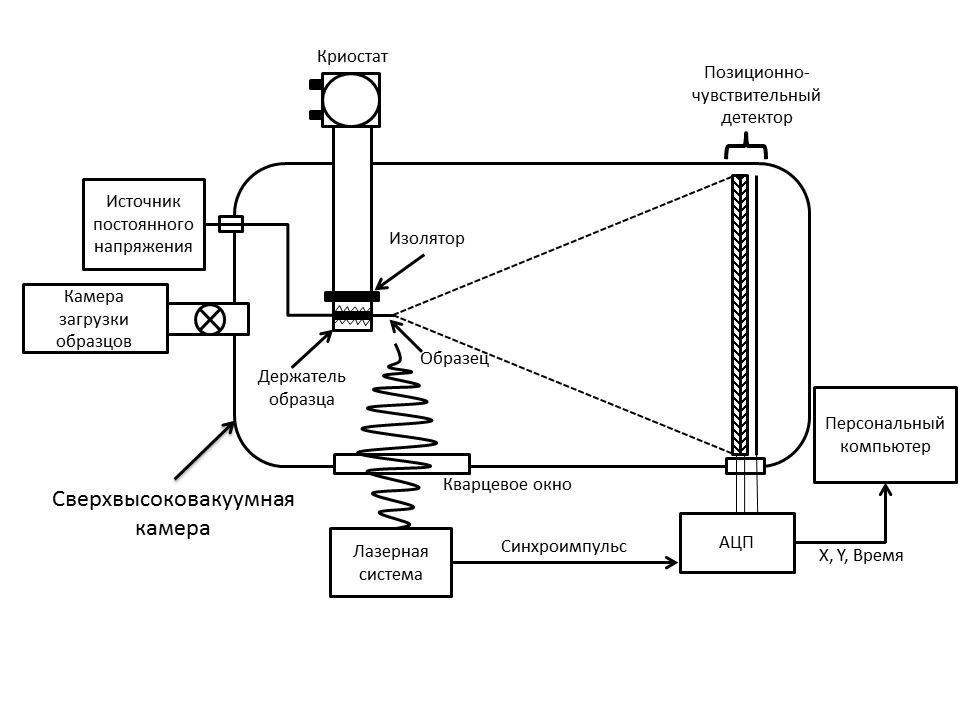
\includegraphics[width=\textwidth]{main_scheme}
	}
	\caption{Схема прототипа атомного зонда ПАЗЛ-3D с лазерным испарением и детектором на линиях задержки}
	\label{fig:main_scheme}
\end{figure}
  
Другой особенностью прямо-пролетной схемы установки можно назвать использование простых алгоритмов восстановления данных. Поскольку в приборе отсутствуют системы отклонения ионов, то траектории пролета можно рассчитывать не прибегая к сложным вычислениям электрических полей на пути пролета иона. Данная особенность важна, когда установка разрабатывается впервые и необходимо её максимально упростить для тестирования и апробирования общего концепта.

Для проектирования компоновки вакуумных объемов и деталей держателя образцов и использовалась система автоматизированного проектирования(САПР) CATIA Dassault Systemes (Франция). К преимуществам данной системы можно отнести: одно из лучших ядер 3Д, возможность быстро и удобно оперировать сборками в сотни деталей и наличие большого количества учебных материалов и пособий. Ниже на Рисунке \cref{fig:APPLE_CAD} показан внешний вид установке на одном из этапов проектирования.
\begin{figure}[htb]
	\centerfloat{
		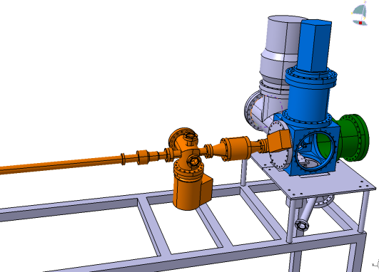
\includegraphics[width=\textwidth]{APPLE_CAD}
	}
	\caption{Внешний вид установки ПАЗЛ-3D в системе САПР CATIA на одном из этапов разработки. Оранжевым цветом выделена камера загрузки с транспортным штоком и шибером, синий - криосистема и часть анализационного объема, зеленый - фланец с расположенной внутри вакуумной частью детектирующей системы}
	\label{fig:APPLE_CAD}
\end{figure}

Как и любой современный микроскоп или томограф АЗТ нуждается в специальном программном обеспечении. Причем необходима разработка собственного ПО управления установкой и сбора на ней данных, так как разрабатываемая установка имеет отличные от зарубежных аналогов узлы. Также наиболее оптимальным решением является разработка собственного ПО для восстановления данных.


\FloatBarrier

\section{Вакуумная и криогенная системы}\label{sec:ch2/sec2}

Одна из основных и важнейших систем в атомно-зондовом томографе - вакуумная система. В АЗТ необходимо поддерживать сверх высокий вакуум для работы детектора и для того, что бы была возможность детектировать отдельные ионы. В общем случае чем выше вакуум создает система, тем лучше. Минимально необходимый уровень вакуума считается равным $10^{-7}$ Торр. Но обычно стараются поддерживать от $10^{-9}$ Торр для уменьшения уровня шума. Для некоторых материалов уровень вакуума критически важен, например, для исследования образцов, в составе которых есть водород или титан.
Ввиду необходимости высокого вакуума система имеет 2 камеры: загрузочную и анализационную. Анализационная камера находится всегда в откаченном состоянии. Откачка вакуумных объемов производится с помощью двух и трех ступенчатых систем насосов. Форвакуумная часть системы представлена двумя спиральными сухими насосами Edwards XS35 (Великобритания), которые обеспечивают разрежение порядка $10^{-3}$ Торр. Далее на загрузочной камере высокий вакуум обеспечивает один турбомолекулярный насос Pfeiffer Vacuum HiPace 300. Уровень вакуума в загрузочной камере находится в пределах от $10^{-7}$ до $10^{-9}$ Торр. Откачку анализационного объема обеспечивают два последовательно установленных турбомолекулярных насоса Pfeiffer Vacuum HiPace 80 и Pfeiffer Vacuum HiPace 1200 (Германия), которые в итоге позволяют поддерживать вакуум до $10^{-11}$ Торр (при включенной криогенной системе). На Рисунке \cref{fig:APPLE_foto_main} представлен внешний вид установки ПАЗЛЗ-3D. Измерение уровня вакуума производится с помощью вакуумметров Thyracont VSH (Германия).

\begin{figure}[htb]
	\centerfloat{
		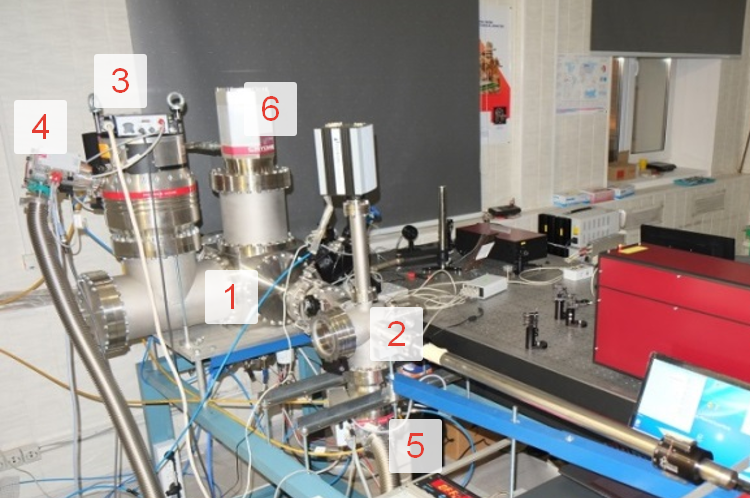
\includegraphics[width=\textwidth]{APPLE_foto_main}
	}
	\caption{Внешний вид установки ПАЗЛ-3D.Цифрами обозначено: 1 - анализационный объем, 2 - загрузочная камера, 3 - турбомолекулярный насос Pfieffer Vacuum HiPace 1200, 4 - турбомолекулярный насос Pfieffer Vacuum HiPace 80, 5 - турбомолекулярный насос Pfieffer Vacuum HiPace 300, 6 - криогенная система CryoMech PT805}
	\label{fig:APPLE_foto_main}
\end{figure}

\FloatBarrier
В качестве криогенной системы выбрана двух-ступенчатая криоголова CryoMech PT805 (США)  типа пульсационная труба. Мощность первой ступени составляет 8 Вт при 20 К, мощность второй ступени 40 Вт при 80 К. Криосистема способна обеспечить минимальную температур 8 К. Но ввиду того, что между криосистемой и образцом находятся держатель патрона образца и монтажные медные проставки, то минимальная температура на образце составляет 20 К. На Рисунке \cref{fig:APPLE_cryosystem} показана криосистема вместе с держателем образца и криоголовой.

\begin{figure}[htb]
	\centerfloat{
		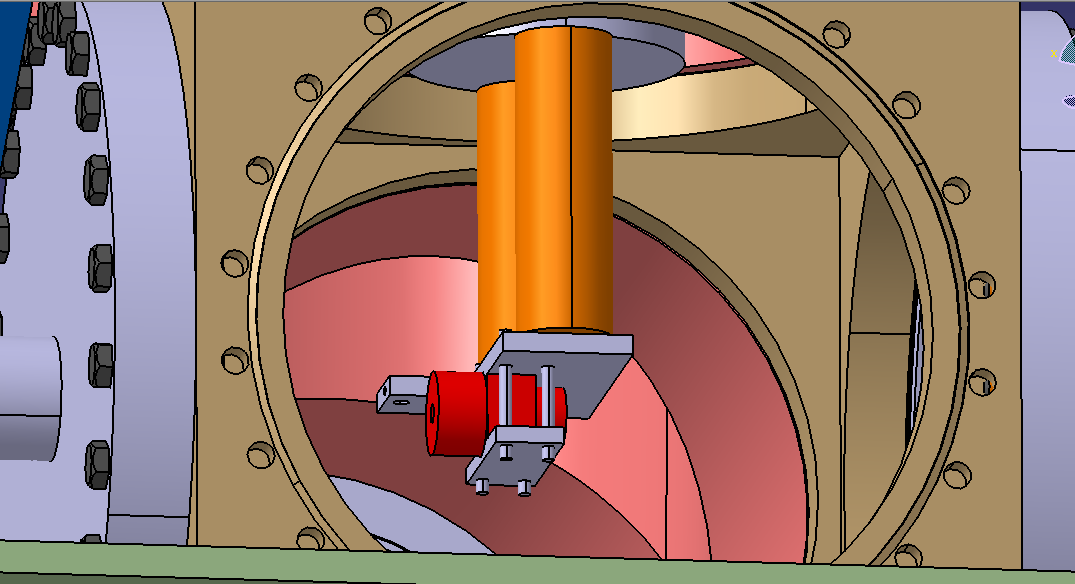
\includegraphics[width=\textwidth]{APPLE_cryoholder}
	}
	\caption{Изображение криоголовы и держателя образца в САПР}
	\label{fig:APPLE_cryosystem}
\end{figure}

\FloatBarrier

\section{Система испарения}\label{sec:ch2/sec3}

Как было выше сказано, для ПАЗЛ-3D было выбрано лазерное испарение. Соответственно, была заказана специальная лазерная система TETA-25ST производства ООО "Авеста-Проект" (Россия), состоящая из нескольких модулей. Основной блок лазера генерирует излучение с длиной волны 1030 нм и длительностью импульса 300 фс. Полная мощность лазерной системы составляет 3 Вт. Энергия импульса составляет от 0,1 до 250 мкДж. Частота работы системы составляет 50 кГц. На Рисунке \cref{fig:APPLE_lasersystem} показа внешний вид лазерной системы.

\begin{figure}[htb]
	\centerfloat{
		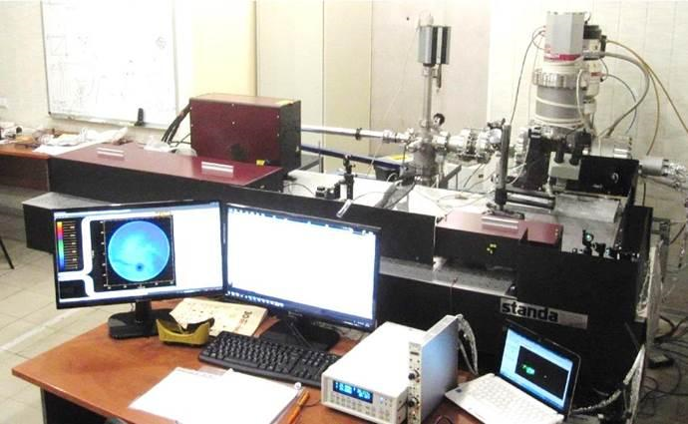
\includegraphics[width=\textwidth]{APPLE_lasersystem}
	}
	\caption{Лазерная система ПАЗЛ-3D ПОМЕНЯТЬ КАРТИНКУ}
	\label{fig:APPLE_lasersystem}
\end{figure}

В системе используется капиллярный компрессор лазерных импульсов. Его принцип работы заключается в уширении спектра входящего лазерного импульса при его распространении в кварцевом капилляре, заполненном инертным газом ксеноном. В дальнейшем спектрально-уширенный импульс сжимается по времени при многократном отражении от чирпированных зеркал. Чирпированное зеркало представляет собой зеркало с многослойным диэлектрическим покрытием, при отражении от которого возникает задержка во времени для импульса с различными длинами волн. После компрессора длительность импульса может составлять от 30 до 60 фс в зависимости от настройки. Далее лазерное излучение опадает в сепаратор гармоник, где происходит генерация второй (515 нм) или третьей (343 нм) или четвертой (257 нм) гармоник. Вторая гармоника имеет наибольшую мощность, что позволяет исследовать материалы при более широком диапазоне возможных энергий импульса. Третья и четвертая гармоники используются для получения более качественных данных при исследовании диэлектриков и полупроводников \cite{Gault06}.

Для испарения атомов (ионов) на образец подается постоянное напряжение с помощью источника высоковольтного напряжения марки FuG Electronik GmbH (до 13 кВ). Лазерное излучение фокусируется с помощью системы линз на кончик образца-иглы. Луч лазера заводится в камеру исследования с помощью системы зеркал и шаговых двигателей, обеспечивающей точность позиционирования менее 2 мкм. Введение лазерного луча в вакуумный объем проводится через специальное кварцевое окно с коэффициентом пропускания более 99\% для любой из 3-х гармоник. Также лазерная система генерирует синхроимпульс для измерения времени пролета частиц, который далее подается на вход модуля АЦП в детектирующей системе.
 Картинка


\FloatBarrier

\section{Детектирующая система}\label{sec:ch2/sec4}

В качестве базового варианта был выбран детектор производства RoentDek GmbH DLD120 с эффективным диаметром 120 мм, так как данная немецкая фирма производит наиболее современные позиционно-чувствительные детекторы на основе линий задержки для детектирования ионов. Детектирующая система состоит из сборки микроканальных пластин (МКП) и системы анодов, усилителя сигнала с детектора и аналого-цифрового преобразователя (АЦП) для оцифровки и передачи данных на компьютер. Схематичное изображение и принцип формирования сигнала при детектировании столкновения иона показан на рисунке \cref{fig:APPLE_detectionsystem} Оцифровка проводится с частотой дискретизации 5 ГГц для сигнала с МКП и с частотой 1 ГГц для сигналов с анодов. 

Принцип детектирования \cite{Spillman00} основан на линиях задержки и состоит в следующем. Ускоренный в поле вблизи образца ион попадает в канал МКП, порождает облако электронов, далее электроны попадают на систему анодов, наводя в проволоке анодов ЭДС. Затем сигнал усиливается в модуле усиления и передается на АЦП.

\begin{figure}[ht]
	\begin{minipage}[b]{0.49\textwidth}\centering
		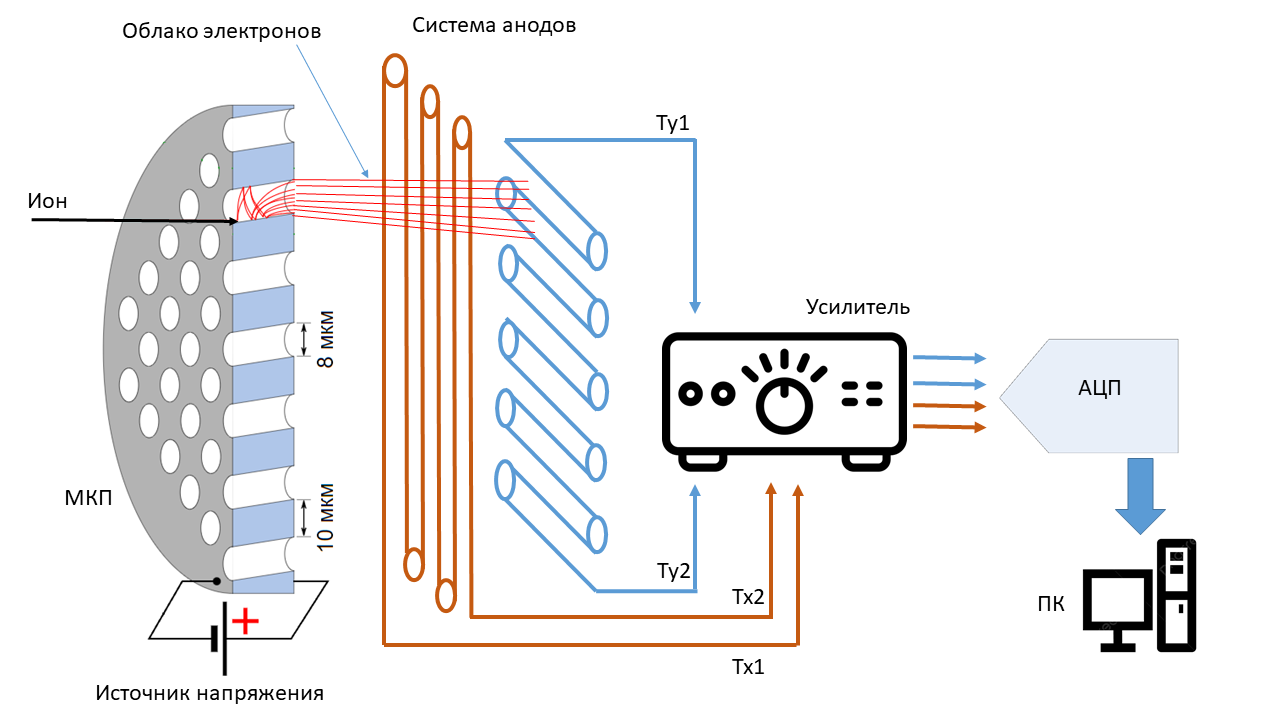
\includegraphics[width=\textwidth]{APPLE_detectionsystem} \\ а)
	\end{minipage}
	\begin{minipage}[b]{0.49\textwidth}\centering
		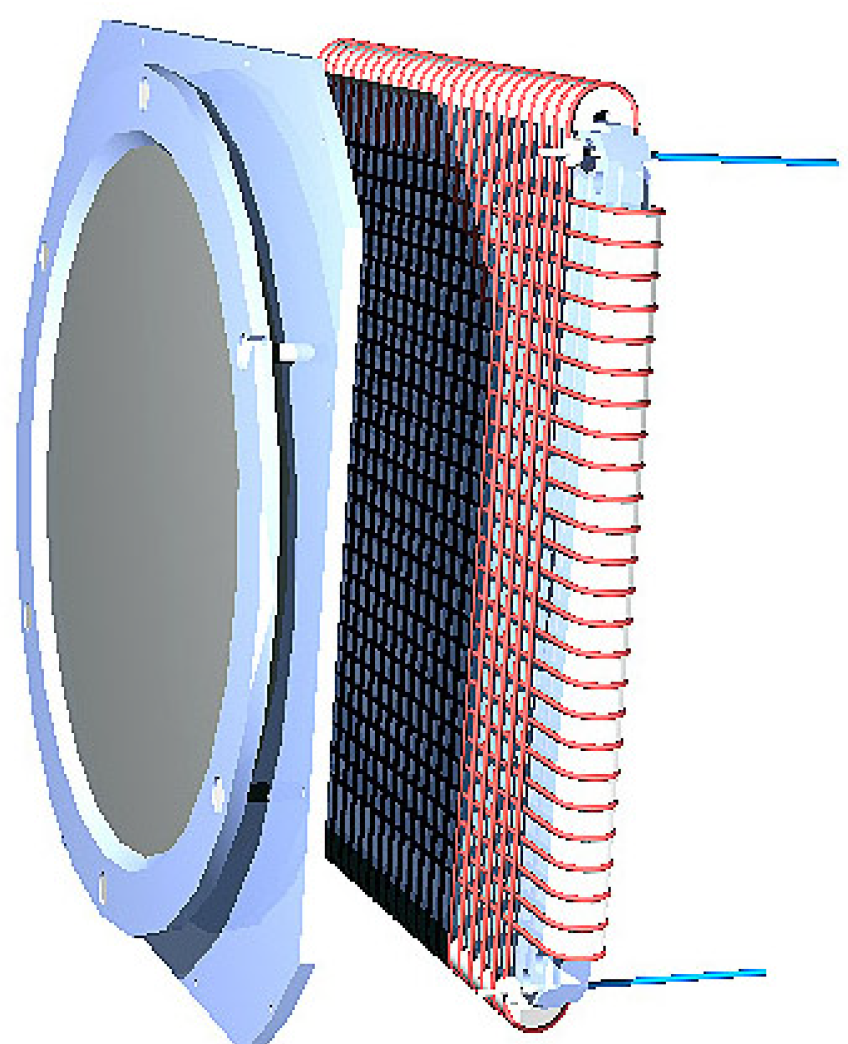
\includegraphics[width=\textwidth]{APPLE_detector} \\ б)
	\end{minipage}
	\caption{Схема работы детектирующей системы. а) Вверху показано столкновение иона с МКП, затем в МКП образуется облако электронов. Ниже показано, как падающее на аноды облако электронов формирует сигнал на выходе. б) Схематичное изображение детектирующей сборки МКП и анодов.}
	\label{fig:APPLE_detectionsystem}
\end{figure}


Координаты прилета частиц на детекторе определяются с точностью менее 100 мкм, что позволяет обеспечить пространственное разрешение прототипа, близкое к атомарному (область образца с характерным размером 100 нм ставится в соответствие области детектора 120 мм). Имеющаяся эффективная площадь детектора в 120 мм при длине пролета ионов 183 мм позволяет достичь угла сбора данных 32, что сопоставимо с аналогичными установками.

\FloatBarrier

\section{Программное обеспечение для управления сбором атомно-зондовых данных}\label{sec:ch2/sec5}

Основное требование к данному программному комплексу 
В рамках разрабатываемого лабораторного образца комплекса атомно-зондовой томографии необходим комплекс программ ЭВМ для управления, сбора.
Основные задачи данного ПО:
Сбор данных с АЦП подключенного к детектирующей системе
Управления напряжением, задаваемым высоковольтной системой на образце
Мониторинг показателей вакуума в различных узлах установки
Управление узлами установки при помощи интерактивной схемы
Мониторинг потока событий с возможностью коррекции текущего напряжения в зависимости от его величины
Мониторинг распределения событий на позиционно чувствительном детекторе
Мониторинг событий на масс-спектре для предварительного анализа химического состава исследуемого образца

Программа сбора данных и управления лабораторным образцом атомно-зондовой томографии ЛабОбр-сбор (далее ПО) является настольным приложением для персонального компьютера. Работа с приложением производится в операционной системе Windows. Управление ПО производится посредством взаимодействия с графическим пользовательским интерфейсом (GUI) после запуска приложения путем запуска файла с расширением .exe. Данная программа разработана в среде разработки Visual studio при помощи компилятора mvsc x64 2015, с использованием библиотек Qt 5.15.2, qwt, и других свободно распространяемых библиотек или библиотек, шедших в комплекте с поставляемым оборудованием. Начальное окно интерфейса ПО представлено на рисунке 4.13.

рисунок ПО

описание картинки 3д, слежение за напряжением, слежение за потоком


Задачи обработки данных:
1) загрузка
2) 3Д восстановление
3) масс-спектр
4) поиск кластеров
5) проксиграммы
6) частотные анализы
7) взаимодействие с БД

Картинки примера обработки


\FloatBarrier

Заключение к главе - собран атомно-зондовый томограф, уникальный для России, преимущества:
- концепт, схема, ПО, логика работы - всё сделано своими силами
- лазерное испарение
- собственное ПО сбора и обработки данных










